\documentclass[xcolor=dvipsnames]{beamer} % dvipsnames gives more built-in colors
\usepackage[utf8]{inputenc}
\usetheme{CambridgeUS}
\usecolortheme{seagull}
\setbeamertemplate{caption}[numbered]
\setcounter{tocdepth}{1}
\setbeamercolor{itemize item}{fg=darkred!80!black}

\usepackage{textcomp}
\usepackage{amsmath}
\usepackage{hyperref}

% Image & figures
\usepackage{graphicx}
\usepackage[labelfont=bf]{caption}
\usepackage{subcaption}
\usepackage{wrapfig}

% Cool tables?
\usepackage{booktabs, tabularx}
\usepackage{multirow}
\usepackage{multicol}
\newcolumntype{b}{X}
\newcolumntype{m}{>{\hsize=.75\hsize}X}
\newcolumntype{s}{>{\hsize=.5\hsize}X}

% Notes
\usepackage{pdfpcnotes}

% Introduction slides before sections and subsections
\AtBeginSection[]
{
	\begin{frame}[noframenumbering, plain]
		\frametitle{Table of Contents}
		\tableofcontents[currentsection]
	\end{frame}
}

\title[EEGSignal]{Characterization of EEG signals according to brain regions using machine learning techniques}
\author[Lai Khang Duy]{Lai Khang Duy \texorpdfstring{ \\ [4mm] 
		{\small \textit{Supervisors}: Sebastian Basterrech}}{}}
\institute[]{ICT Department - University of Science and Technology of Hanoi}
\date{August 16, 2019}

\begin{document}
	\frame{\titlepage}
	
	\begin{frame}
		\frametitle{Table of Contents}
		\tableofcontents
	\end{frame}

	\section{Introduction}
	
	\begin{frame}{Brain}
		\begin{figure}
		    \centering
		    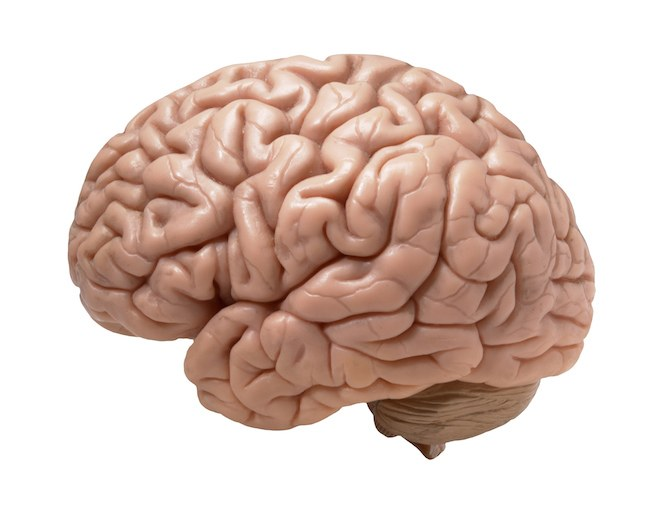
\includegraphics[width=0.7\textwidth]{images/brain1.jpg}
		    \caption{Human brain}
		    \label{fig:brain}
		\end{figure}
	\end{frame}
	
	\begin{frame}{Introduction}
	    \begin{itemize}
	        \item Every vertebrates and most of invertebrates have brain.
	        \item When it works, it generates electrical signal.
	        \item Electroencephalography (EEG) is a method to record the neuraloscillations (often known as "brain waves") of the brain.
	        \item Different region of the brain generates specific type of different signal.
	    \end{itemize}
	\end{frame}
	
	\begin{frame}{Problem and Objective}
	    \begin{itemize}
	        \item \textbf{Objective: }Characterize brain regions over labeled EEG signal.
	        \item \textbf{Why we have to study this?}
	        \begin{itemize}
	            \item When some area of the brain is damaged, the brain plasticity provokes other parts. It can be activated and have new functionalities in order of mitigating the impact of brain damages. 
	            \item So here is why:
	            \begin{enumerate}
	                \item Analyzing the plasticity of the brain.
	                \item How damaged brain provokes changes in their functionality.
	            \end{enumerate}
	        \end{itemize}
	        \item Our goal is to have a general comparison between 2 well-known machine learning techniques LSTM and SVM in classifying brain regions. 
	    \end{itemize}
	\end{frame}
	
	\section{Theoretical background}
	
	\begin{frame}{Brain electrical signals}
	More specific
		\begin{itemize}
		    \item Brain is a complex organ, contain over 86 bilions neurons.
		    \item Each neuron connects to thousands of others.
		    \item Communicate over synapses electrical signal.
		\end{itemize}
	\end{frame}
    
    \begin{frame}{Electroencephalography}
        \begin{columns}
        \begin{column}{0.5\textwidth}
            \begin{itemize}
            \item Frontal lobe (F) (Red)
            \item Cerebellum (C) (Cyan)
            \item Parietal lobe (P) (Yellow)
            \item Occipital lobe (O) (Emerald)
            \item Temporal lobe (T) (Green)
            \end{itemize}
        \end{column}
        
        \begin{column}{0.5\textwidth}
            \begin{figure}
                \centering
                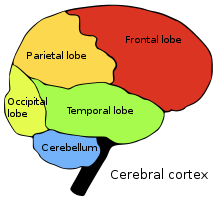
\includegraphics[scale=0.7]{images/Brain.png}
                \caption{Region of the brain}
                \label{fig:region}
            \end{figure}
        \end{column}
        \end{columns}
    \end{frame}
    
    \begin{frame}{Electroencephalography}
        \begin{columns}
        \begin{column}{0.5\textwidth}
            \begin{figure}
                \centering
                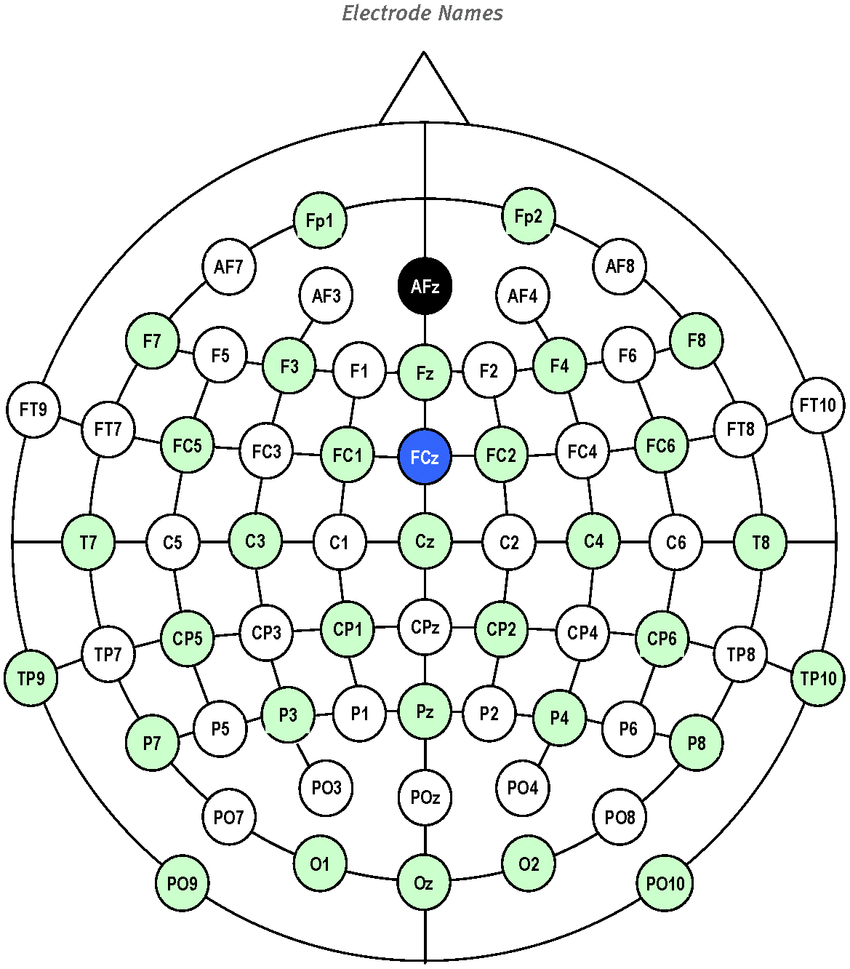
\includegraphics[scale=0.13]{images/EEG_electrodes_map_full.png}
                \caption{full electrode map system}
                \label{fig:full}
            \end{figure}
        \end{column}
        
        \begin{column}{0.5\textwidth}
            \begin{figure}
                \centering
                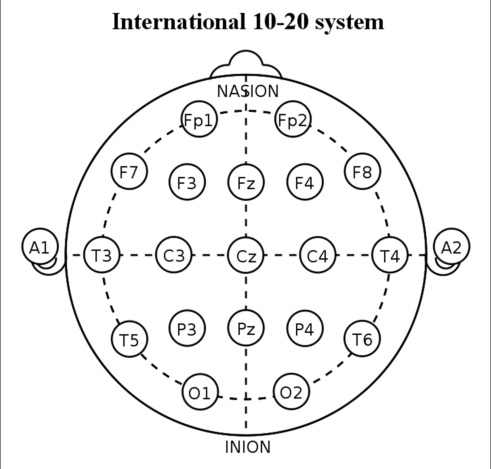
\includegraphics[scale=0.55]{images/EEG_electrodes_map_19.png}
                \caption{19 electrodes map system}
                \label{fig:19}
            \end{figure}
        \end{column}
        \end{columns}
    \end{frame}
    
    \begin{frame}{Electroencephalography}
        \begin{figure}
            \centering
            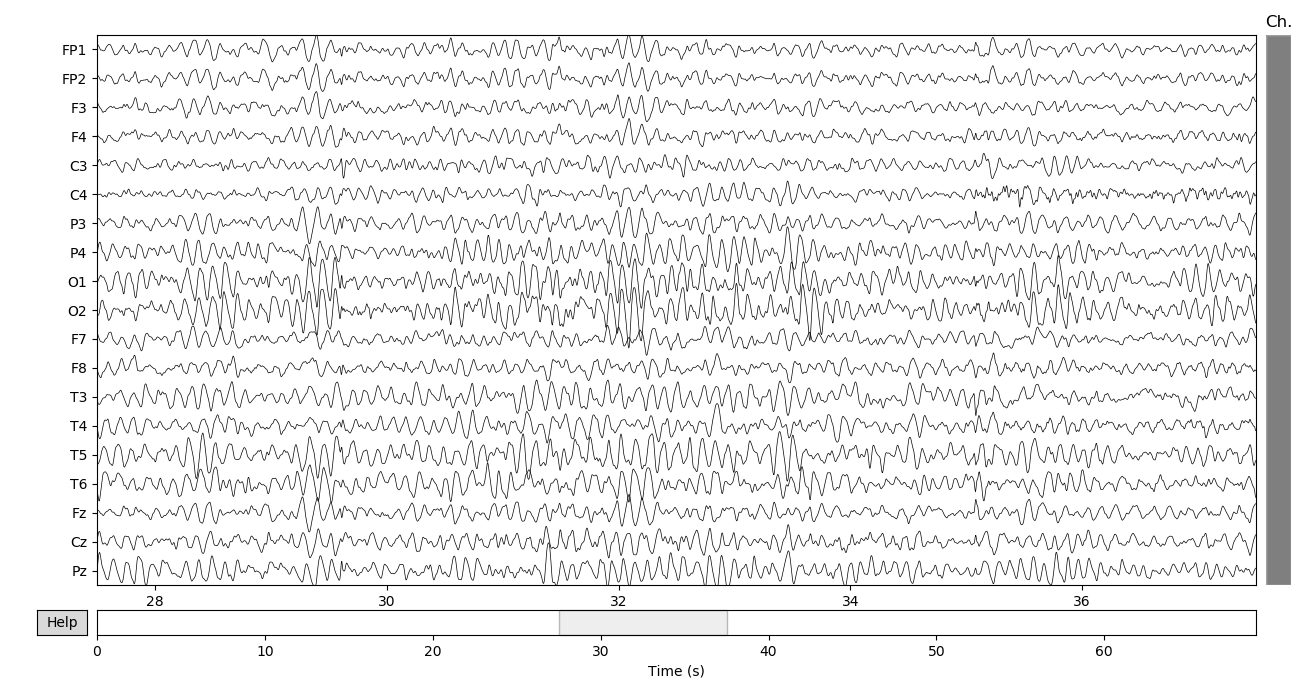
\includegraphics[scale = 0.25]{images/EEG_with_MNE.png}
            \caption{19 EEG signal example}
            \label{fig:fulldisplay}
        \end{figure}
    \end{frame}
    
	\section{EEG signals pre-processing}
	
	\begin{frame}{EEG signals pre-processing}
		To have the data ready for the machine learning part, we have to get through:
		\begin{itemize}
		    \item Noise reduction
		    \item Learning set creation
		\end{itemize}
		
		\begin{figure}
	        \centering
	        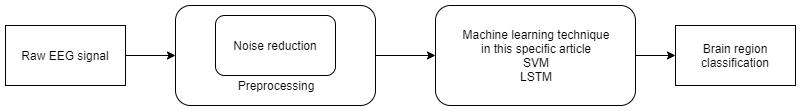
\includegraphics[scale = 0.4]{images/GeneralDiagram.png}
	        \caption{Project sequences breakdown}
	        \label{fig:breakdown}
	    \end{figure}
	\end{frame}
	
% 	\begin{frame}{EEG signals pre-processing}
% 	    \begin{figure}
% 	        \centering
% 	        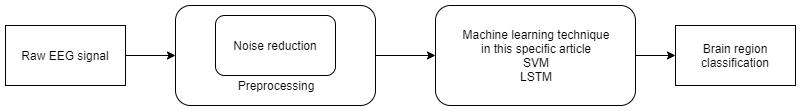
\includegraphics[scale = 0.4]{images/GeneralDiagram.png}
% 	        \caption{Project sequences breakdown}
% 	        \label{fig:my_label}
% 	    \end{figure}
% 	\end{frame}
	
	\begin{frame}{Noise reduction}
	
	The technique that we use to denoise in this study is Z-score.
		$$z={{x-\mu}  \over \sigma }$$
		
	\textbf{Why ?}
	
	Because EEG signal very stable. Any significant changes is considered as outliers. In this case, I want to consider around 5\% of the data we have is outliers.
	\end{frame}
	
	\begin{frame}{Noise reduction}
	    \begin{figure}
	        \centering
	        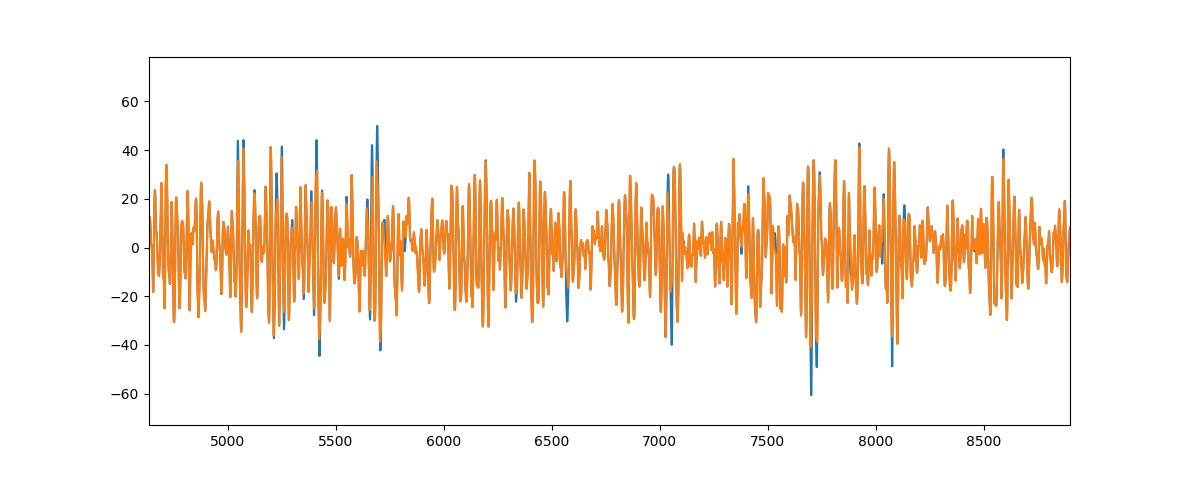
\includegraphics[scale=0.4]{images/fp1-2.png}
	        \caption{FP1 before and after apply Z-score}
	        \label{fig:FP1}
	    \end{figure}
	\end{frame}
	
	\begin{frame}{Noise reduction}
	    \begin{figure}
	        \centering
	        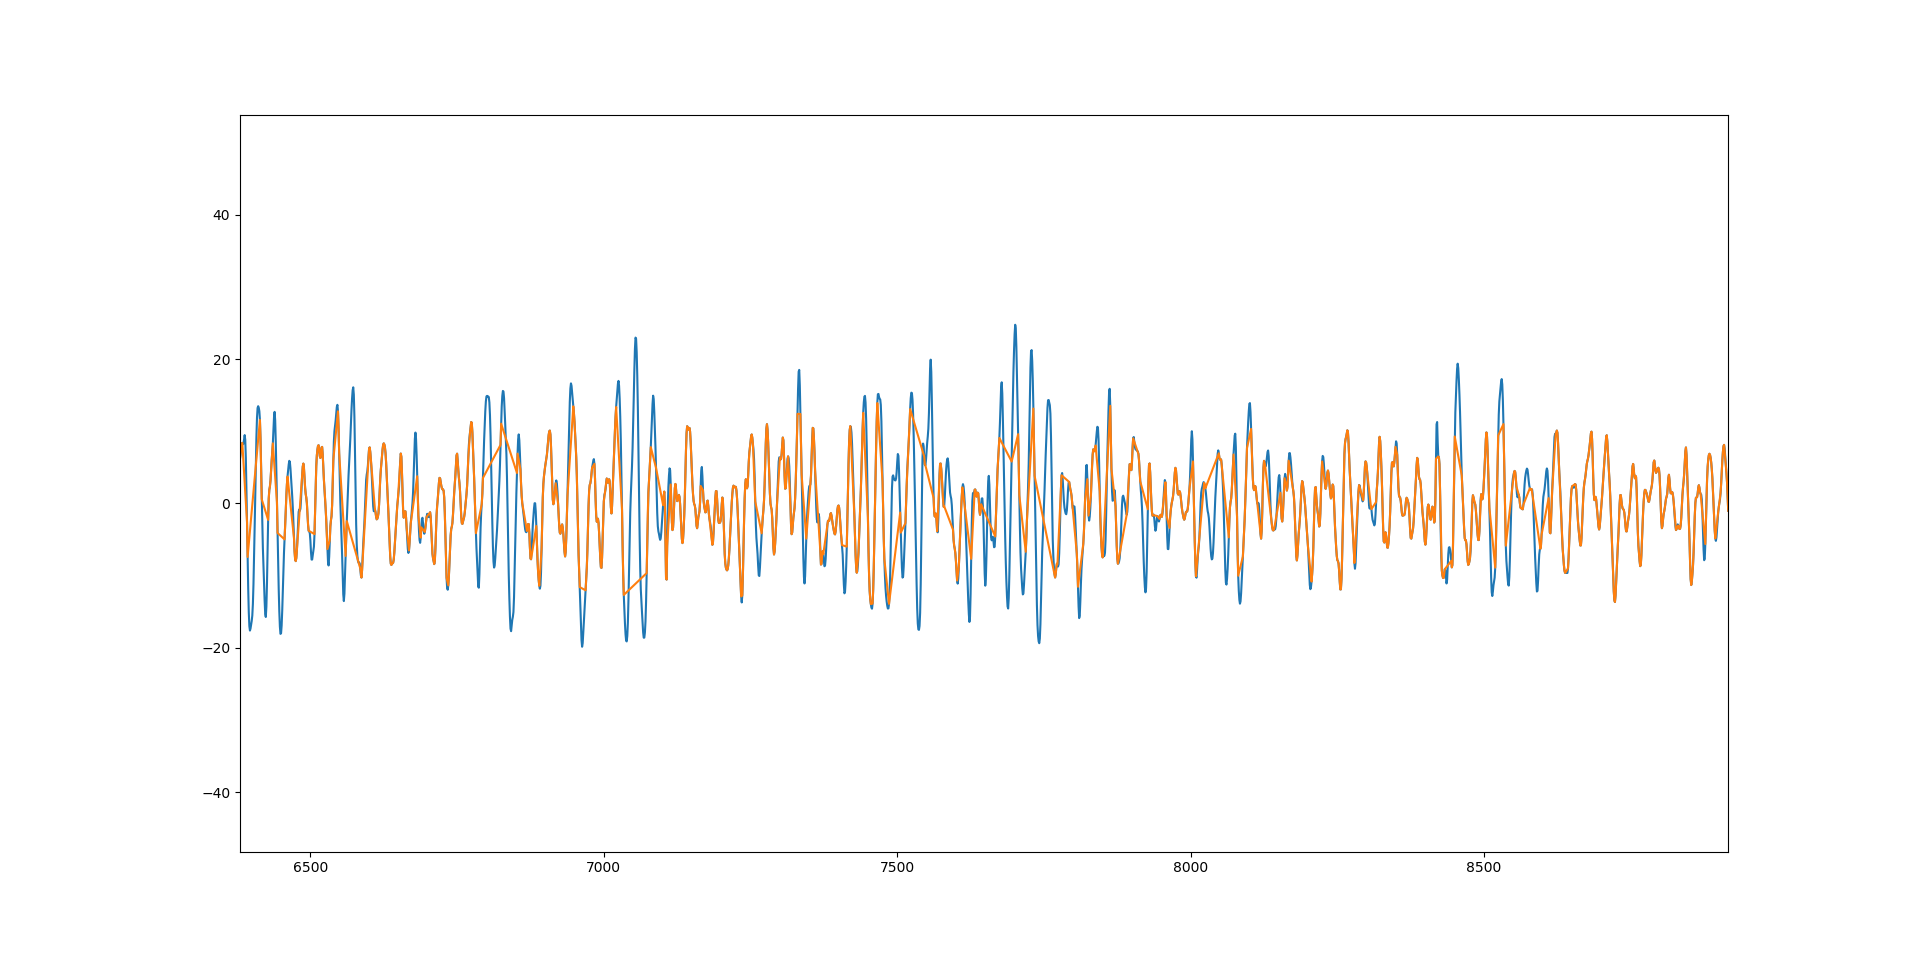
\includegraphics[scale=0.23]{images/Figure_1.png}
	        \caption{Closer look at FP1 before and after apply Z-score}
	        \label{fig:FP1close}
	    \end{figure}
	\end{frame}
	
	\begin{frame}{Learning set creation}
	    \begin{itemize}
	        \item 19 electrodes
	        \item 4 classes:
	            \begin{enumerate}
	                \item Class 0: including FP1-AVE, FP2-AVE, F3-AVE, F4-AVE, F7-AVE, F8-AVE, Fz-AVE
	                \item Class 1: including C3-AVE, C4-AVE, Cz-AVE
	                \item Class 2: including T3-AVE, T4-AVE, T5-AVE, T6-AVE
	                \item Class 3: including P3-AVE, P4-AVE, Pz-AVE, O1-AVE,  O2-AVE
	            \end{enumerate}
	        \item 2 datasets with the same signal:
	            \begin{enumerate}
	                \item W1: 200 time steps
	                \item W2: 400 time steps
	            \end{enumerate}
	       \item Shuffle whole dataset after divide classes and time windows.
	    \end{itemize}
	\end{frame}
	
	\begin{frame}{Learning set creation}
	    2 same datasets with different time window
	    \begin{itemize}
	        \item W1: 200 time steps each datapoint
	        \item W2: 400 time steps each datapoint
	    \end{itemize}
	\end{frame}
	
	\section{Machine learning methods}
	
	\begin{frame}{LSTM-RNN}
		\begin{figure}
		    \centering
		    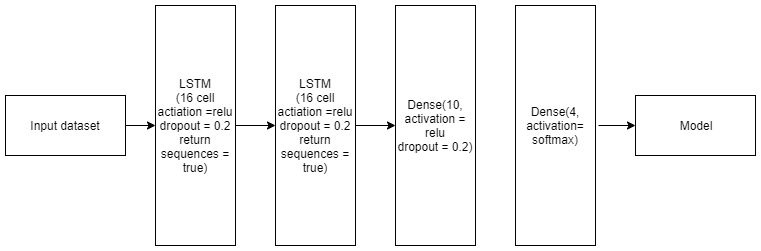
\includegraphics[scale = 0.45]{images/LSTMDiagram.png}
		    \caption{LSTM neural network breakdown}
		    \label{fig:my_label}
		\end{figure}
	\end{frame}
	
	\begin{frame}{SVM}
		\begin{itemize}
		    \item Implement SVC in scikit-learn
		    \item Parameter:
		        \begin{enumerate}
		            \item Gamma: scale
		            \item C: 100
		        \end{enumerate}
		\end{itemize}
	\end{frame}
	
	\section{Empirical results}
	
	\begin{frame}{LSTM-RNN}
	    \begin{table}[]
            \begin{tabular}{|l|l|}
            \hline
                      & W2 = 400                        \\ \hline
            Epoch 1/2 & acc = 0.3173, val\_acc = 0.4255 \\ \hline
            Epoch 2/2 & acc = 0.3387, val\_acc = 0.4326 \\ \hline
            \end{tabular}
            \caption{Accuracy using LSTM with window W2=400 time steps}
        \end{table}
        
        \begin{table}[]
            \begin{tabular}{|l|l|}
            \hline
                      & W1 =200                        \\ \hline
            Epoch 1/2 & acc = 0.1941, val\_acc = 0.2626 \\ \hline
            Epoch 2/2 & acc = 0.2662, val\_acc = 0.3805 \\ \hline
            \end{tabular}
            \caption{Accuracy using LSTM with window W1=200 time steps}
        \end{table}
	\end{frame}
	
	\begin{frame}{SVM}
	    \begin{table}[h]
            \centering
            \begin{tabular}{|l|l|}
            \hline
            W2 = 400        & W1 =200          \\ \hline
            accuracy = 0.72 & accuracy = 0.575 \\ \hline
            \end{tabular}
            \caption{Accuracy using SVM with windows W1=200 and W2=400 time steps}
            \label{table:SVM}
        \end{table}
	\end{frame}

	\section{Conclusion and future works}
	
	\begin{frame}{Conclusion}
	    \begin{itemize}
	        \item SVM has better accuracy than LSTM-RNN.
	        \item window W2 has better accuracy than window W1.
	        \item 0.72 is our best results by far.
	    \end{itemize}
	\end{frame}
	
	\begin{frame}{Future works}
	    It is still possible to improve the classifier. We have figured out some of the reasons might affect the result:
	    \begin{itemize}
	        \item Lack of data.
	        \item ECG and EOG still have not be removed.
	        \item Try to change the filter.
	    \end{itemize}
	\end{frame}
	
\end{document}